\documentclass[a4paper,11pt]{report}

%   _____  _____  ______          __  __ _      ____  ______ 
%  |  __ \|  __ \|  ____|   /\   |  \/  | |    |  _ \|  ____|
%  | |__) | |__) | |__     /  \  | \  / | |    | |_) | |__   
%  |  ___/|  _  /|  __|   / /\ \ | |\/| | |    |  _ <|  __|  
%  | |    | | \ \| |____ / ____ \| |  | | |____| |_) | |____ 
%  |_|    |_|  \_\______/_/    \_\_|  |_|______|____/|______|

\usepackage[utf8]{inputenc}
\usepackage[backend=bibtex]{biblatex}
\bibliography{../Dissertation}
\usepackage{graphicx}
\usepackage{tabularx}
\usepackage{longtable}
\usepackage{xcolor}
\usepackage{wrapfig}
\usepackage{setspace}
\usepackage{datetime}
\usepackage{url}
\usepackage{tikz}
\usepackage{pgf-umlsd}
\usepackage{pgfgantt}
\usepackage{pdflscape}
\usepackage{pdfpages}
% \usepackage{showframe}
\usepackage{geometry}
\geometry{
 a4paper,
 left=1in,
 top=1in,
}
\newcommand{\titles}{\\\vspace{1cm}}
\newcommand{\cn}{\textcolor{red}{[Citation Needed]}}
\newcommand{\objv}[3]{\item \textbf{OBJ-#1}: \textit{#2}\\#3}
\newcommand{\objitem}[4]{\begin{tabularx}{\textwidth}{lXr} \textbf{OBJ-#1} & #2 & #3\end{tabularx}\\#4\\}
\newcommand{\riskitem}[4]{\begin{tabularx}{\textwidth}{lcr} \textbf{RSK-#1} & #2 & #3 \\  \multicolumn{3}{X}{#4} \\  \end{tabularx}}
\newcommand{\objts}{\multicolumn{3}{X}{}\\}
\newcommand{\gi}[2]{\textbf{#1} - #2}
\newcommand{\todo}[1]{\textcolor{red}{TODO: #1}}


\newcounter{FunCount}
\newcounter{NFunCount}
\newcommand{\freq}[3]{\addtocounter{FunCount}{1}F\arabic{FunCount} & OBJ-#1 & #2 & #3\\}
\newcommand{\nfreq}[3]{\addtocounter{NFunCount}{1}N\arabic{NFunCount} & OBJ-#1 & #2 & #3\\}

\pdfinfo{%
  /Title    (Deliverable 1: Final Year Dissertation - Research Report)
  /Author   (Leon McGregor)
}



%   _____   ____   _____ _    _ __  __ ______ _   _ _______ 
%  |  __ \ / __ \ / ____| |  | |  \/  |  ____| \ | |__   __|
%  | |  | | |  | | |    | |  | | \  / | |__  |  \| |  | |   
%  | |  | | |  | | |    | |  | | |\/| |  __| | . ` |  | |   
%  | |__| | |__| | |____| |__| | |  | | |____| |\  |  | |   
%  |_____/ \____/ \_____|\____/|_|  |_|______|_| \_|  |_|   



\begin{document}
\pagestyle{empty}

{\centering\Large
\includegraphics[width=0.4\textwidth]{../hwu.png}\titles
Final Year Dissertation\\
Deliverable 1 - Research Report\titles
{\huge\bfseries Web Platform for Code Peer-Testing\titles}
L\'eon \textsc{McGregor} - H00152968\titles
{\large\textit{Supervisor}\\}
Manuel \textsc{Maarek}\titles
{\large\textit{Second Reader}\\}
Andrew \textsc{Ireland}\\
\vfill
}

\newpage
{
  \renewcommand{\thispagestyle}[1]{}
  \begingroup
    \makeatletter
    % Redefine the \chapter* header macro to remove vertical space
    \def\@makeschapterhead#1{%
    %\vspace*{50\p@}% Remove the vertical space
    {\parindent \z@ \raggedright
        \normalfont
        \interlinepenalty\@M
        \Huge \bfseries  #1\par\nobreak
        \vskip 40\p@
    }}
    \makeatother

    \tableofcontents
  \endgroup
}
\newpage
\doublespacing


\section*{Abstract}
Undergraduate students in Computer Science courses take part in coursework exercises in the form of programming tasks. The primary aim of this project is to improve this process by facilitating peer testing and peer feedback. The project will achieve this through creation of a website that will let peers assess each others coursework solutions. This document will detail the background research going into this project, and the plan for developing and subsequently evaluating the website.

\vfill

\section*{Declaration}
I, L\'eon McGregor confirm that this work submitted for assessment is my own and is expressed in my own words. Any uses made within it of the works of other authors in any form (e.g., ideas, equations, figures, text, tables, programs) are properly acknowledged at any point of their use. A list of the references employed is included.\par
Signed: L\'eon McGregor\par
Date: \today

\vfill

\section*{Acknowledgements}
Thanks to Manuel Maarek for helping me to organise this project.

\newpage

\pagestyle{headings}
\markright{L\'eon McGregor - Deliverable 1: Final Year Dissertation}

%   _____ _   _ _______ _____   ____  
%  |_   _| \ | |__   __|  __ \ / __ \ 
%    | | |  \| |  | |  | |__) | |  | |
%    | | | . ` |  | |  |  _  /| |  | |
%   _| |_| |\  |  | |  | | \ \| |__| |
%  |_____|_| \_|  |_|  |_|  \_\\____/

\section{Introduction}
In Undergraduate Computer Science courses, students will complete coursework. Some of this coursework may involve programming exercises. This project aims to improve these programming exercises through the involvement of peer assessment. Specifically, peer testing of programs and peer feedback. To facilitate this, the project will create a prototype for a \textit{Web Platform for Code Peer-Testing}.\par
The web platform (referred to as a website) will allow students to engage in peer assessment of each others solutions to exercises (in this case program code) by peer-testing. That is, students will share solutions through the website, view and test solutions for other students, and then give and receive feedback on solutions.\par
Ideally, the peer assessment that takes place within the website will provide more immediate and useful feedback on coursework than having to wait for a teacher, and the results of testing could be used as a starting point for final grading of the coursework assignment.\par

Much research has been already completed in the study of Peer Assessment, peer testing and technology-enhanced learning environments. Some relevant research into this will be analysed within this document, as well as a discussion of related or similar systems that have previously been implemented by others. I will also look into some aspects relating the the implementation of the desired web platform, such as security, and how program testing can be done.\par

There are two high level aims that make up this project:
\begin{enumerate}
\item \textbf{Prototype} - Design and build a website that automates peer assessment - That is to say, it combines file upload, viewing, testing and providing feedback in one place.
\item \textbf{Evaluate} - Prepare and execute an evaluation study into whether or not this website enhances peer assessment - By comparing a peer assessment process with and without this site, I can determine if it can offer any advantages to the users.
\end{enumerate}

\newpage
\section{Overview of Concept}
This is a description of the ideal usage of the website, and identifies some \textit{key terms}:
\begin{enumerate}
 \item A \textit{teacher} (Course Lecturer/Professor) will set a coursework exercise
 \item A \textit{student} on the course will act as a \textit{developer}, and create a \textit{solution} to the exercise
 \item Students will then \textit{upload} the solution to the \textit{website}
 \item Students take on the role of \textit{testers}. This involves creating and submitting \textit{test cases} to the website
 \item The website will silently run these test cases and store the \textit{test results}
 \item Testers can view the test results and the \textit{source code} of the solution
 \item Testers can add feedback based on what they see from the source code and test results
 \item A student can then see the feedback for, and the test cases and test results used on, their submission
 \item A teacher can see all data that has been submitted to the website 
\end{enumerate}
Considering this process in terms of a more traditional peer assessment, the testers and developers would be assessors and assessees respectively.



%   ____          _____ _  _______ _____   ____  _    _ _   _ _____  
%  |  _ \   /\   / ____| |/ / ____|  __ \ / __ \| |  | | \ | |  __ \ 
%  | |_) | /  \ | |    | ' / |  __| |__) | |  | | |  | |  \| | |  | |
%  |  _ < / /\ \| |    |  <| | |_ |  _  /| |  | | |  | | . ` | |  | |
%  | |_) / ____ \ |____| . \ |__| | | \ \| |__| | |__| | |\  | |__| |
%  |____/_/    \_\_____|_|\_\_____|_|  \_\\____/ \____/|_| \_|_____/

\chapter{Background}
\section{Peer Assessment}
\subsection{What is it?}
Peer assessment is a process in which students assess each other. This opposes the more traditional stance where a teacher performs the assessment. As defined by topping \cite{topping_peer_2009},
\begin{quote}
``Peer assessment is an arrangement for learners to consider and specify the level, value, or quality of a product or performance of other equal-status learners.''
\end{quote}
That is to say, students with a similar level of education assessing the work of each other to give critical feedback and discussion. This could be done in many ways, such as between pairs or in groups, and can be performed on any number of different activities from programming exercises to oral reports.


\subsection{Why use it?}
Peer assessment is a process with many benefits to participants in education. Sadler \& Good \cite{sadler_impact_2006} have suggested the following concepts that peer assessment can help with
\begin{itemize}
 \item Peer assessment is more immediate, so students can get more feedback, and sooner
 \item Students performing marking can reduce the workload for teachers
 \item The process of checking and thinking about another students answer can improve a students own understanding
 \item Peer assessment can help students better understand testing and can become aware of their own strengths and weaknesses
 \item Following peer assessment students can gain an improved attitude towards the process of learning as a whole
\end{itemize}
From this, we can see that using peer assessment is definitely a desirable activity to include in the educational process.\par

Peer assessment can offer much help towards education of students, but it would be worthwhile to know just which aspects are the most useful. A study conducted by Li et at. \cite{li_assessor_2010} investigated the peer assessment process with the aim of discovering which part of it is most useful to the students involved: Being an assessor or an assessee. To study this, undergraduate student teachers were given the task of creating a \textit{WebQuest}\footnote{In this context, a \textit{WebQuest} project is an activity created by the student teachers that would be given to their students. Following the \textit{WebQuest} instructions, students are guided through Internet resources, and offered ``scaffolding activities'' to help them learn.} project. This was then marked by independent assessors, and the student teachers were given a chance to provide feedback on other student teachers \textit{WebQuests}. Following this, the feedback was shared back, students teachers were given another chance to improve their project, and it was marked again. The quality of the peer feedback itself was also checked by the independent markers. The study found that 
\begin{quote}
``there was a significant relationship between the quality of the peer feed-back the students provided for others and the quality of the students' own final projects''
\end{quote}
The findings of the investigation would suggest that the actual exercise of providing feedback to others (acting as an assessor) is a worthwhile process for learning from. This study also concluded that there was no reasonable link between the feedback itself as a learning tool, suggesting that the act of giving feedback itself is more valuable and that low quality feedback does not harm the learning experience.\par
From the results of this study, we can gather that the most effective part of peer assessment is the actual act of assessment itself. Therefore, in a system that helps students assess program code, we want to prioritise helping them to perform this assessment over making sure that the feedback the students can provide is useful. Through this, we can ensure that students make the most learning possible out of the system.


\subsection{How to do it?}

With the knowledge that peer assessment can be useful, it is important to know how a peer assessment should be conducted. A study performed in a classroom environment by Smith et al.\cite{smith_using_2012} focused more on the use of peer assessment as a tool for teaching testing of code, in addition to the existing course.\par
Over the course of this study, which took place using coursework from a 12-week university course, the following was completed for each coursework: Submitting solutions, then submitting peer reviews (which includes a description of the testing that they performed on another solution, and the results of this), and then a review of the peer assessment (including what was learned, an evaluation of feedback on their own solution, and optionally a corrected solution).\par
One particularly noteworthy aspect of this use of peer assessment was the double-blind nature, ensuring anonymity. Students would not be aware of who they were marking, or were marked by. To enforce this completely, submitted code was obfuscated (java sources into byte code). One advantage of this is that it strips out identifying variable names and comments, which could identify other students. However, a downside of using byte code is that it can make it difficult to do in-depth analysis of the source structure which may make it harder to write complete test cases.\par
The study identified two key features that assignments for peer assessment need to have:
\begin{itemize}
 \item Well-defined interfaces
 \item Freedom for implementation
\end{itemize}
In addition to this, Smith has found that it was possible to integrate the peer assessment process without having to significantly alter the existing course material, and the students taking part enjoyed the experience. This shows promise, as it could indicate many Computer Science courses (that offer coursework meeting the requirements), could be modified to include their own peer assessment exercises.\par

Peer assessment can prove to be a very valuable experience for students. Falchikov has collected various case studies of past peer assessments \cite{falchikov_improving_2013}, and the following aspects can be found:
\begin{itemize}
 \item If the marking criteria are properly explained, there is often no significant difference between the marks awarded by students and those that would be awarded by teachers. This would tend to indicate that students do assess each other fairly.
 \item One of the most important aspects of peer assessment is the ability of the student to learn how to assess other students and then know how to critically assess and improve their own work as a result.
 \item It is important to make sure students feel confident, otherwise they may not assess their peers as honestly as they might otherwise have done. Some students will feel conflicted about marking their peers, particularly if they might have to give low marks.
 \item During peer assessment more benefits may come from students assessing multiple solutions, rather than each focusing on one.
\end{itemize}

\subsection{Summary of Peer Assessment}
The process of peer assessment holds much value for all of the participants in the educational process, and can provide some skills that can be carried beyond students time in education. It can be used to provide more immediate feedback, help students to learn as they evaluate solutions and create this feedback, and could be integrated with some existing coursework assignments. Beyond just letting students learn about how to grade against a mark scheme, peer assessment can often teach students a lot about the subject material itself, letting them gain a deeper understanding about it. Peer assessment also helps to grow students ability to critically evaluate both their own, and others, work. Students who are to engage in Peer assessment should be given sufficient help so that they can perform the assessment with confidence, and work with multiple peers to get the full positive effects of peer assessment.


% ------
% TECH+ PLATFORM
% BACKGROUND
% -----
\section{Technology-Enhanced Learning Platforms}
\subsection{Virutal Learning Environments}
There has been a rapid increase in the use of websites and internet services in recent times, and many of these services can aid in student learning. One such style of website is the Virtual Learning Environment (VLE). Examples of such websites could include Moodle, \cite{moodle_about_2016} or Blackboard \cite{blackboard_blackboard_2016}. The use of a VLE can be very valuable to students learning, as they offer such features as integrated coursework submission systems, discussion forums, sections for storing and displaying class lecture notes and more.\par
Analysis performed by Mogus et al. \cite{mogus_impact_2012} looked at data collected over two semesters of a teacher education course. The study then collected bulk data regarding usage statistics from the various tools offered by Moodle (the VLE of choice in the study). During analysis, this data was correlated against the success of students in that course, as measured by their final grade. The analysis 
revealed that the interactions used within the VLE do have a positive influence on the eventual grades a student receives. It is worth noting this was not determined by using a control group, but by grouping students by their final grade, and then analysing the results.\par
Given that VLEs can be useful to students, and that the desired peer assessment system would be an online website, it seems that a logical aim would be to build a peer assessment system that is modular enough that it may be integrated into such a VLE as Moodle.\par

To determine whether students can benefit from peer assessment in an online, \textit{technology-enhanced}, environment, a research project was conducted by Keppel et al. \cite{keppell_peer_2006}. This project involved some university lecturers, who re-structured their courses to involve more peer learning, with the aid of a virtual learning environment (in this case, Blackboard).\par
The project took place over 3 different case studies. The different studies used journal, discussion and filesharing features of the VLE to enhance 2 courses in fashion design, art education and the design of a new learning website. Based on the evidence collected during these case studies, it was found that:
\begin{itemize}
 \item Students found this assessment to be fairer than just against teacher
 \item Students appreciated the ongoing peer critique performed through the reflective journals
 \item Teachers felt the instant nature of feedback was very useful
 \item The support offered by the assisting technology of the VLE encouraged collaboration
\end{itemize}
The authors of the project also suggest that unless the peer assessment within the VLEs is a marked process (against a students grade), students may be unwilling to participate. These findings are quite useful, and are a good indicator that the positive aspects of traditional peer assessment are not hindered by using an online system (as opposed to in-person activities).\par

\subsection{Classroom Platforms}
A study by Phil Davies\cite{davies_computerized_2000} was conducted using a peer testing system in a university communications and networking module. This peer testing system aimed to help students easily provide feedback on reports, in addition to attempting to locate plagiarism.\par
The CAP (Computerized Assessment with Plagiarism) provided an interface to let students read the report of another student. They could then provide feedback on the report and follow references on the report to identify any \textit{copy \& paste} plagiarism. This CAP system is of particular interest as the web interface described in Davies' paper is quite similar to what I would aim to produce during this project. Although this Davies' system is more aimed at identifying plagiarism in reports than testing program code, I do feel that this is still relevant as it makes use of a quite involved peer assessment process.\par
This experiment followed the results students achieved over a sequence of 4 tasks:
\begin{enumerate}
\item A Report
\item A multiple choice test
\item A period for peer marking the reports between students
\item A final multiple choice test
\end{enumerate}
The experiment looked to see if the peer marking was at all helpful in improving the marks of students between the two tests. The results found that the peer marking was very useful for students who had initially performed poorly. Student comments on the experience would suggest that they found the peer assessment process both enjoyable and informative. There is also evidence from this feedback indicating the importance of maintaining anonymity, as some students felt it would be difficult to the marking non-anonymously.\par
From this, I can gather that the model of peer assessment used, through the web interface, was indeed successful. Based on the evidence from this study, the use of a similar system could well be helpful to students who would otherwise not have performed well. This study also revealed that students learned a lot from the ``repetitive nature of the marking''. This could indicate that testers in such a system as mine might benefit from testing multiple solutions.\par
Given that the user interface and flow of information through the application provided by CAP is in many ways similar to my conceptual website, I would have liked to obtain a copy of it to evaluate further. Unfortunately, Davies has not made the source for the website available for download.\par
\begin{wrapfigure}{R}{0.4\textwidth}
\centering
\includegraphics[width=0.35\textwidth]{CAP.png}
\caption{\footnotesize A sample view of the CAP system, showing report viewer and marking guide.}
\end{wrapfigure}


In the 1990s, the University of Nottingham produced Ceilidh, a system that had the intent of automating and improving the assessment process for C Language Coursework. Later improvements were made by Heriot-Watt University adding support for
Standard ML (SML) \cite{foubister_automatic_1997}. This tool was used to guide students through the coursework, and then check the correctness of submissions. Ceilidh offered a skeleton answer to students, which pointed out any special language features that should be used. The submitted solutions are checked for correctness with a mixture of verifying output against a model solution, and checking the style of the code (e.g line count, use of certain function names, etc).  In particular for SML, students were asked to provide the types for written functions, as an additional test of understanding.\par
A study conducted by Foubister et al. investigated if such a system used for automatic assessment of students would be useful. To check this, the results of the final exam mark were compared to those marks from previous years where Ceilidh was not used. The study found that there was no real improvement made by Ceilidh, but most importantly there were no detrimental effects. Some positive side effects were observed: The time taken for students to receive feedback on the coursework was markedly decreased, and the tracking of progress offered by the tool allowed teachers to more easily identify any students that were having serious difficulties.\par
Given that I wish to implement a system that is more geared towards peer assessment rather than automated assessment, I think that the most valuable idea to draw from this would be the tracking that is offered to the teacher. Even though it is the students who will be doing the actual assessment, teachers should be able to see how students are progressing with these.\par

In 2002, M. Goldwasser started a peer testing initiative on a Data Structures course \cite{goldwasser_gimmick_2002}.  The main objective of this was to get students taking the course to submit, along with coursework, a test case to run on the program with the aim of finding bugs in other students programs. The main objective in this case was to focus learning on software testing, and the peer testing aspect was secondary, however the study does hold many parallels with my intended system design.\par
The submitted coursework solutions would be collected, along with each test case. Then, using an automated system each of the test cases would be run against each of the solutions. The major downside to this being that there is $x^2$ complexity in terms of the submission count.\par
Goldwasser offers some advice for potential future implementations of such an automated testing system:
\begin{itemize}
 \item To prevent some students falling behind due to having buggy input parsers, have the lecturer provide a standard implementation to to all students. Similarly, output needs to be handled in a standardised way.
 \item A limit should be placed on how large a test case a student can submit.
 \item the automated testing system should be able to handle the case where a solution works correctly, produces the wrong output, crashes, or does not terminate.
 \item Additionally, the testing system should be able to recover and restart from a given position without having to re-run all test cases, or re-run specific test cases if one of the submissions should change
\end{itemize}
I believe this advice is quite useful for our purposes. If building such a system, it is worthwhile to know and consider the various states a program could exit with when running the tests cases. This is still useful even if the implementation I create does not perform a full running of each test to each solution. The suggestion that the lecturer provide a way to handle input and output in a standard way is useful, but more so for lecturers who will set coursework assignments for the website.\par
Additionally, Goldwasser left the autograder used within his study open for download \cite{goldwasser_autograde_2002}. This script could be used as a starting point for implementation of running test cases. However, it does seem to offer more than I require, such as automatically grading (beyond just verifying test cases), and checking against a model answer.

\subsection{Contest Platforms}
As an aside to peer assessment, one optional feature of such an implementation could be to offer automated testing. If a lecturer so wished, they could use the system with a pre-submitted test case. In effect, acting as a peer to each student, so that they could recieve test results immediately (or as quickly as the test completes) upon submission.\par
The effectiveness of an automated testing tool (as a sole means of feeback, outside peer assessment) was investigated Farnqvist \& Heintz \cite{farnqvist_competition_2016} within a Data Structures Course.\par
This study investigated how introducing a competitive element to a Data Structures and Algorithms CS course might help students to learn. The survey took place over two runs of the course over 2011 and 2012. In the 2011 course, lab contests were graded manually, and a voluntary contest used an automated grader. In the 2012 course, the lab assignments were marked using an automated grader for testing correctness and efficiency, and by human lab assistants to check code quality. The automated grader in use was \textit{Kattis} \cite{enstrom_five_2011}\par
This test showed the attitudes of some students towards the use of an automated grader. Students found this automated grading to be more fair than the manual equivalent. The study also found that ``students put in more effort in the course thanks to automated assessment''. This would suggest that allowing my implementation to be configured to run as an automated tester might be a worthwhile addition.\par
For the competitive element of this, the study found that competition positively affected student behaviour. The element that was most useful for the contest aspect of this was the autograder. The auotmated marking and tracking of marks proved useful in motivating students, by offering a leaderboard.\par


Build-it, Break-it, Fix-it\cite{ruef_build_2016} is a programming contest that uses the concept of a Peer testing system to judge the success of various programming assignments. This success is measured both in terms of general correctness and specifically in the context of security. This is somewhat different to the aim of an educational peer assessment website, however it is worth mentioning as the implementation used by the project is, I believe, a good starting model for my implementation of a web platform.\par
\begin{wrapfigure}{l}{0.4\textwidth}
\centering
\includegraphics[width=0.35\textwidth]{bibifi.png}
\caption{\footnotesize Basic diagram showing the architecture of the BiBiFi contest system.}
\end{wrapfigure}
The contest requires participants to \textit{build} a working solution that matches functional specifications, as well as being as secure as possible. If the solution can be built and the functionality verified by an automated system, then the team can move on to the next stage. Following this, testers will attempt to \textit{break} the security of the solution, and points will be allocated according to a zero-sum-game. The builders can then gain points by \textit{fixing} their solutions.\par
Throughout the contest, there is a central web-based infrastructure that manages running the contest website (with scoreboards, etc.), listening to builder git repositories, and also running and recording test results. The basic structure is as follows:
\begin{enumerate}
 \item There is a listener component that tracks changes to the git repo of the builders
 \item This pulls metadata to the contest database
 \item The database can activate and get results from the tester component
 \item The tester can use Amazon EC2 to create virtual machines which run the solution, and the tests, then check the results against a benchmark and oracle to see if all is correct (or not)
 \item after reporting this back through the tester to the database, the website front end will update any scoreboards
\end{enumerate}
The basic architecture described here seems to work very well for the contest, and I believe with some modification would be a good starting point for my own implementation. There is no need for git repositories, as the files are uploaded directly to the system. This could just represent the servers filesystem. Also, while a VM creation system might work well for the contest, I feel that this might be too costly, in monetary terms and time overhead. A simpler sandboxing solution might make more sense, particularly if the system is password protected and only used by students who probably don't want to risk losing coursework marks.

\subsection{Summary of Tech-Enhanced Platforms}
There are many advantages, with respect to learning, brought forward by technology enhanced platforms. Some, such as web-based VLEs are more accessible, allowing students to take part in collaborative exercises from outwith the time and space constraints of a classroom. In Computer Science classrooms, technology is often used to aid in the automation of program testing. This can have positive effects such as giving quicker feedback on solutions and more accurately checking the correctness of solutions with many inputs. These tools could also provide more feedback to the teacher of a class, such as the progress being made by students, to help identify any problems. These systems can also be useful in contests, outwith classrooms and within. Within classrooms, contests using such systems can encourage students to perform better. Such systems can also evoke ideas for how a new technology enhanced learning system could be implemented. This includes the style of architecture, the interfaces that could be used and the general flow of the applications in use.\par



% ------
% IMPLEMENTATION
% BACKGROUND
% ------

\section{Implementation Considerations}
From the previous sections we can see that there is definitely a space for a website to aid in peer testing code. However, there are many issues to consider when choosing how the website should be developed and implemented.

\subsection{Anonymity}
One issue that can arise when students are interacting with each other from a perspective of evaluating each other is their anonymity. During a peer assessment / automated testing experiment performed by Sitthiworachart et al. \cite{sitthiworachart_effective_2004}, the students remarked about the use of anonymity. One students response suggested that in a non-anonymous peer assessment exercise, their marking would be influenced if they knew who it was they were marking. Another student said they would decline to take part if the peer assessment was not conducted anonymously. What can be drawn from these comments is that anonymity is clearly very important to those taking part in the peer assessment. But the opinions of anonymity might not correlate with the actual effect it has.\par

To study the effect that anonymity has, as opposed to just opinions about it, a study was conducted by Lan Li \cite{li_role_2016}. This study aimed to investigate just how effective anonymity is when it comes to making peer assessment more effective, and whether any negative impact from a lack of anonymity can be mitigated.\par
This quasi-experimental study was conducted with some in-training teachers, and aimed to see which is the most effective method of / using / while conducting a peer assessment exercise: Having assessors and assessees know each others identities, remain anonymous, or know identities while having received training. The training in this case involved watching a video that described some of the stresses and concerns that arise during peer assessment, and various forms of discussion regarding this.\par
One issue I have with this study is that it didn't cover the case of being anonymous and getting training. This was because the training was intended as a fallback for when anonymity is not possible. But this does invite the question of just how effective would anonymity be if training were offered as well.\par
The study found:
\begin{quotation}
\begin{enumerate}
 \item ``Anonymity improves student performance in peer assessment''
 \item If anonymity can't be guaranteed, negative effects arising from this can be offset using training
 \item Anonymity does not reduce the pressure and tension related with peer assessment
\end{enumerate} 
\end{quotation}

From the evidence available, I can gather that there is a great importance in creating a peer assessment system which can function while maintaining anonymity. It might also be worthwhile integrating some form of training, as found in the study by Lan Li, as this might reduce stress during the peer assessment process, as it is not outwith the real of possibility that students might recognise the work of others even if it is anonymous.

\subsection{Security \& Sandboxing}
If the website we aim to create is going to integrate built-in running of test cases we will need to make sure to use the right way of doing this. Because the website we aim to build will accept solutions from students that will need to be executed, it is important that these applications be restricted in terms of the permissions available to them. Restricting how they can interact with the executing computer will prevent malicious attacks or accidental errors in code from damaging the whole system.\par
Some available security measures include AppArmor, SELinux, FBAC amongst others. A study by Schreuders \cite{schreuders_empowering_2011} investigated how easy it is to set up the relevant security measures. They found that the FBAC-LSM security model was the best in terms of the ease of setting up, and ensuring that programs worked correctly. The tool offered for FBAC-LSM security set up would be a good candidate for use in a peer assessment system for running programs.\par
There is also the idea of running programs directly in a browser, using a JavaScript interpreter in a way such as PyPy.js \cite{pypy.js_web_2016}. In this manner, the local file system would be protected, as the filespace used by the python interpreter is virtual in memory. However this would not be an ideal solution, as if there were security risks they would simply be placed upon the assessor instead. Additionally, this model of execution would make it more difficult to get and store results of tests and would need to be run synchronously in the website UI. Long operations also block the browser from functioning (having tried this myself, I can see that this would be an issue).\par
Another method might be to modify source codes to use a language-specific sandboxing features. One example of such an interpreter/compiler is PyPy\cite{pypy_pypy_2016}, which is designed to offer some sandboxing. However, this is still in development and could not be relied upon for our purposes.\par
One issue with sandboxing security mechanisms is that such systems can only protect the system by blocking access certain API calls. To put it another way, sandboxes cannot in and of themselves identify malicious code. For this reason it might be worth integrating some form of anti-malware analysis as well.\par
As an alternative to sandboxing, one common method is to re-map the root directory to prevent an application from accessing files on the system that it should not. This is known as a chroot jail \cite{ubuntu_basic_2016}. This could be a useful way of restricting the solution submitted so that it can only read the relevant files (e.g. compilers/interpreters).

\subsection{Testing Submitted Solutions}
When considering the testing of software, there are several ways that this can be done. To produce a website that enables peer assessment, an appropriate testing methodology will need to be selected. Based on suggested testing styles from Bill Laboon \cite{laboon_friendly_2016}, some testing methodologies were considered for inclusion:
\begin{itemize}
 \item Linting - Performing basic checks for 'smells' of bad code design, such as identifying unused variables or methods. Not particularly useful from a perspective of checking code is correct, but is still useful in terms of producing good quality code.
 \item Unit testing - The use of xUnit style tests. Often used in test-driven development, these could be useful in detecting flaws if written post-development by a peer assessor. This would need the assessor to be familiar with how to write xUnit style tests, and how they should be structured, or it would not be viable.
 \item Expected output testing - Running a program with some input and comparing the output to what is expected. The issue here is that the peer assessor first needs to know what the correct output is. Unlike unit testing, this would simply involve a series of inputs, and a series of expected outputs, and the task of checking the correctness from these tests is left to the website.
 \item Scenario Testing - Simulate an actual usage scenario. Assessors would use solutions as if they were 3rd party libraries (a 'black box'), and develop their own programs that would use these as if in an actual use case. These programs would perform checks to make sure the solutions being tested were running as expected. This is more involved than unit or expected output testing, as it might be better placed to discover side effects of continued use of the solution.
 \item Property based testing - Using a proof checker, such as QuickCheck (or a similar implementation for languages other than Haskell) to ensure that a program is acting correctly. This would place additional overhead onto the students as assessors, as they would need to learn and understand the annotations used by a proof checker, but could provide a lot of coverage of possible inputs.
\end{itemize}
In all cases, the solution being tested needs to conform to a standard interface. And in each case, the website running the tests needs to be able to extract some meaningful information. This is simpler in terms of unit and expected output, as these will offer output that will be easily readable (e.g. by diff, a count of pass/fail tests); scenario and property based tests would produce more verbose output, which while may be more informative, would be harder to analyse and subsequently summarise. 

\subsection{Recording Feedback}
In addition to recording the results of test cases, to enable full peer assessment beyond just peer testing, the desired website should integrate methods of providing feedback through testers critical evaluation of solutions. There are many different ways this could be achieved however, beyond just receiving and recording a paragraph or two of text from the tester.
\subsubsection*{Inline Code Annotations}
One feature seen in Agile software development cycles is the Code Review \cite{github_project_2016}. This involves a colleague reviewing new code, and leaving comments for improvements. GitHub enhances this process by offering inline code annotations. These allow for feedback to be more targeted and, from this, likely easier to understand. This could be a useful feature to implement, as student testers could leave comments for the developers where necessary in the code.
\subsubsection*{Marking Against Criteria} 
To once again draw on research conducted by Falchikov \cite{falchikov_improving_2013}, they discuss peer assessment traits in terms of the criteria used to mark other students. There are different levels of input that students can receive while engaging in preparations for peer assessments. The teacher may provide all of the criteria for marking/assessing; there may be discussion between the students and teachers, where each decide what criteria are important; and lastly offering full control of the criteria to mark over to students. In an open ended answer situation, as is offered by programming exercises, this may be a good environment to encourage the student to come up with more of the criteria.\par
Given a criteria to mark against, it would be useful to integrate some simple systems to check that a given solution meets the defined criteria. Falchikov describes that some common methods used are likert scales or checklists, working against a known criteria.

\subsection{Summary of Implementation Considerations}
Given the many different aspects covered above, I have identified the following key considerations when implementing the website:
\begin{itemize}
 \item A desirable outcome would be to have a website that can operate without any students knowing the identities of the students whose code they are testing and assessing.
 \item It will be important to impose some form of security on the website. There are many measures that could be taken here, including sandboxing mechanisms, that is restricting the operating system access of the executable; running an executable in a more secured environment, such as a jail; or including malware detection software.
 \item There is a choice of methods to employ when creating test cases. The test cases testers will write could include linting, unit testing and scenario testing, amongst others.
 \item Feedback could be collected from the testers through free comment in various places of the application, or by checking against a marking criteria.
\end{itemize}





%            _____ __  __  _____ 
%      /\   |_   _|  \/  |/ ____|
%     /  \    | | | \  / | (___  
%    / /\ \   | | | |\/| |\___ \ 
%   / ____ \ _| |_| |  | |____) |
%  /_/    \_\_____|_|  |_|_____/ 

\chapter{Project Aims}
\section{Primary Aim}
The primary motivation of this project, as stated in the introduction, is to improve the student experience when completing programming coursework exercises by facilitating peer learning. The main aims for the project derived from this can be stated as:
\begin{enumerate}
\item \textbf{Prototype a Website}\par
Design and build a website that automates peer assessment. This website should combine all the tasks that would normally have to be done manually by students and allows them to be completed from a website interface. This could include file uploads, file viewing, testing of programs and providing feedback. The objectives for the Prototype are broken down further in the next section (\S2.2).
\item \textbf{Evaluate the Website}\par
Once a functioning prototype is created, perform a study to determine the effectiveness of the website in terms of how well it enhances peer assessment within the confines of the coursework. This evaluation should involve students who might potentially use this tool in a course. The exact properties we wish to ensure the website has are expanded upon in the evaluation section, \S3.1.
\end{enumerate}

\section{Prototype Objectives}
These are the objectives that relate to the Prototyping of the peer testing website. These are further broken down into requirements in the later section on implementation (\S4.1).
\objitem{Upload}{File upload for solutions}{High Priority}{The website will let students upload solutions to assignments.}
\objitem{Test}{Build test cases}{High Priority}{The website will let students build, and subsequently submit test cases in a simple way. As previously discussed in \S1.3.3, possible implementations of this subsystem include many different forms of testing, such as Unit Testing, Property based testing and more.}
\objitem{Run}{Run test cases}{High Priority}{Once the test cases are built, run them. The results of running them will be stored for later display. This is done asynchronously to the main interface, as running the test cases may take some time. This could extend to running a submitted test against all solutions.}
\objitem{View}{Viewing own solution}{High Priority}{Let the student see their own submission, which test cases have been run against it, the status of each test, any feedback from peer assessors.}
\objitem{Results}{Display test results}{High Priority}{Display the results of a test against a particular solution. Display the results (passed, failed, error, metadata?) on each test.}
\objitem{Security}{Secure the System}{Medium Priority}{As the website acts as an open interface for running python, it is important that it be secured against attacks (malicious or accidental), and that only the relevant people may access it.\par
While in a production system, security would normally hold a high priority, in this prototype stage, the focus will be more so on the functionality that evaluation test subjects will interact with. Given that this evaluation will be monitored, test subjects can be prevented from uploading malicious code. However, this prototype will need to have some form of authentication in place, to make sure that only developers and test subjects may access the website.}
\objitem{Feedback}{Provide feedback on solution}{Medium Priority}{A tester should be able to provide feedback to the developer at various stages of the assessment. This could include at the results of tests or on the source code.\par
An ideal implementation of this would provide a way for testers to give feedback to the solutions, within certain places of the peer assessment. Possible objectives that could interact with feedback include:
\begin{itemize}
 \item OBJ-Results: Once tests are run, the tester could attach comments to the (results of) test cases
 \item OBJ-Source: Annotating the source code of solutions (possibly on a line by line basis, or by leaving general comments for a submitted solution)
 \item OBJ-Teacher: A teacher should be able to view all of the feedback that has been submitted by testers, in all the appropriate places
\end{itemize}~}
\objitem{Source}{Show source code}{Medium Priority}{A tester should be able to read the source code of a solution, for example to inspect the coding style (variable names, structure etc.)}
\objitem{Teacher}{Teacher overview screen}{Low Priority}{Provide a way for the teacher of the class to set the coursework. Also, to see all of the solutions and the tests run on each of them, as well as any feedback.}
\objitem{Modular}{Create a modular system}{Low Priority}{One motivation for building the system would be to plug it into other learning tools, such as moodle.}
\objitem{Record}{Record metadata about run solutions}{Low Priority}{When running solutions with test cases, record metadata such as time taken to complete, memory usage, code coverage, etc. Store this data for display with each test result.}


%   ________      __     _     _    _      _______ _____ ____  _   _ 
%  |  ____\ \    / /\   | |   | |  | |  /\|__   __|_   _/ __ \| \ | |
%  | |__   \ \  / /  \  | |   | |  | | /  \  | |    | || |  | |  \| |
%  |  __|   \ \/ / /\ \ | |   | |  | |/ /\ \ | |    | || |  | | . ` |
%  | |____   \  / ____ \| |___| |__| / ____ \| |   _| || |__| | |\  |
%  |______|   \/_/    \_\______\____/_/    \_\_|  |_____\____/|_| \_|

\chapter{Evaluation Strategy}

\section{Evaluation Properties}
In order to test if the website is useful or successful, we wish to test for and see if the following properties are true:\\
\begin{tabularx}{\textwidth}{lX}
 \textbf{EVA-Share} & The process of sharing source code and test cases is A) easier and B) faster in a web interface as opposed to sharing via traditional means such as a file system or email.\\
 \textbf{EVA-Automate} & The automation of running test cases against source codes, and recording/displaying results is: A) Correct, B) Faster than performing this manually.\\
 \textbf{EVA-Enhance} & The feedback that is given through the website is as useful as, or better, than that given without the website.\\
 \textbf{EVA-Improve} & Subjectively check if test subjects feel that the peer assessment process is improved by using the website.\\
\textbf{EVA-Secure} & Just how secure is the system in its current prototype state. Are there any flaws that could be exploited, and what possible steps could be taken to mitigate against these.
\end{tabularx}

\section{Test Strategy}
In order to evaluate whether each test property has been met, a good strategy would be to:
\begin{enumerate}
 \item Use a simple programming exercise, e.g. a Binary Search Tree
 \item Have test subjects perform the peer assessment each others solutions without the website
 \item Test subjects respond to questionnaire regarding this process
 \item Perform a different programming exercise, e.g. An auto-balancing Binary Tree
 \item Have test subjects again perform a peer assessment but this time with the website
 \item Test subjects respond to questionnaire regarding this process
 \item Test subjects may then attend a discussion session to debrief after completion
\end{enumerate}
I feel the evaluation would need to be performed in this way (with subjects both using the website, and not using it), as in order to test \textbf{EVA-Improve}, as you can only really gauge how the subjects feel about the website if they have tried both with and without it. The issue with testing in this manner is one of learning. As subjects will have completed one task already, their opinions and ability may be skewed by the second task. To mitigate this, we would want to swap the order in which both the tasks and the use of the website occurs (ideally this requires a minimum of 4 pairs of test subjects).\par
In order to test \textbf{EVA-Share}, we can test this by A) Observing how files are shared, and seeing if the test subjects understand the website and the website works correctly, and B) timing how long it takes to share files with and without the website.\par
\textbf{EVA-Enhance} can be tested by A) asking the users which feedback they found more useful, and also by B) having the markers (in this case the evaluation test runner) assess and compare the feedback itself, on a more objective level: How detailed is it, Is the feedback correct, etc.\par
\textbf{EVA-Automate} is similar in some ways to \textbf{EVA-Submit}, and could use the same evaluation methods, but in addition it is necessary to check that the tests themselves are actually correct and useful. It is possible that the website may guide and improve, or hinder, the production of meaningful test cases during the peer assessment.\par
Regarding \textbf{EVA-Secure}, I do not feel it would make sense to analyse the security of the system by including other test subjects. Given that the prototype is likely to be deployed on a live system (at Heriot-Watt university), an analysis performed theoretically rather than practically would be desired.\par
This analysis should cover potential security flaws in terms of potential malicious code students might upload, exploits that could allow students (or other unauthorised actors) to access the system in unintended ways, and also seeing that the running of the website does not interfere with the rest of the live system it will be running on.

\section{Test Subjects}
The test strategy would require pairs of 2. At least 4 pairs (To count each combination of With/without website and task1/task2). It would be useful if the student has some prior knowledge of using python to program, but not be totally necessary. At least some proficiency in an object-oriented language would be needed.

\section{Feedback}
Students will be invited to complete a questionnaire at key points during the evaluation study. This will help to gauge the immediate reaction to using the system. Also, depending on numbers of involved participants, there may be an open answer discussion session held once the experiment is complete, where participants are invited to openly discuss how they feel about the concepts covered.

\section{Ethical Analysis}
The ethical analysis form for this evaluation study is included as an appendix. This details any ethical issues that might arise from the study, recruiting participants, and handling data. This ethical analysis has been approved by the Project Supervisor and the University Ethics Coordinator.


%   _____  ________      ________ _      ____  _____  __  __ ______ _   _ _______ 
%  |  __ \|  ____\ \    / /  ____| |    / __ \|  __ \|  \/  |  ____| \ | |__   __|
%  | |  | | |__   \ \  / /| |__  | |   | |  | | |__) | \  / | |__  |  \| |  | |   
%  | |  | |  __|   \ \/ / |  __| | |   | |  | |  ___/| |\/| |  __| | . ` |  | |   
%  | |__| | |____   \  /  | |____| |___| |__| | |    | |  | | |____| |\  |  | |   
%  |_____/|______|   \/   |______|______\____/|_|    |_|  |_|______|_| \_|  |_|

\chapter{Development Plan}

\section{Requirements}
Based on the objectives outlined in \S 2.1, I can establish the following system requirements:\par
The following prioritisation is used:\\
\begin{tabular}{ccc}
 Low & Mid & High\\
 Possible future addition & Would make a more useful system & Necessary for prototype
\end{tabular}

\begin{longtable}{cclr}
\textbf{ID} & \textbf{Objective} & \textbf{Description} & \textbf{Priority}\\\hline
\freq{Security}{Log students in}{High}
\freq{Security}{Log teachers in}{Low}
\freq{Upload}{Accept student uploads of solutions to assignments}{High}
\freq{Test}{Accept uploads for test case files}{High}
\freq{Test}{Offer a more guided approach to writing test cases}{Mid}
\freq{Run}{Run submitted test case for the submitted solution}{High}
\freq{Run}{Record the results of test execution}{High}
\freq{Run}{Run submitted test case against all solutions}{Low}
\freq{View}{List all test case submitted}{High}
\freq{View}{Display the results of running a test}{High}
\freq{View}{Display the results of all solutions test run against}{Low}
\freq{Results}{Let submitter of test see the results}{High}
\freq{Source}{Let tester see source code of solution}{Mid}
\freq{Feedback}{Let submitter of test add/edit feedback}{Mid}
\freq{Feedback}{Record testers general comments on solution}{Mid}
\freq{Feedback}{Let tester attach feedback to lines in solution}{Low}
\freq{Security}{Sandbox the execution of solutions}{Mid}                                                                                                                               
\freq{Security}{Use malware detection to prevent malicious uploads}{Mid}
\freq{Teacher}{Let teacher set coursework assignments}{Low}
\freq{Teacher}{Let teacher see all submitted content}{Low}
\nfreq{Website}{Operate on Desktop Web Browsers used in classroom}{High}
\nfreq{Website}{Operate with multiple users accessing at once}{High}
\nfreq{Website}{Operate with a classroom of users accessing at once}{Low}
\nfreq{Upload}{Accept solutions that are python scripts}{High}
\nfreq{Run}{Test cases should be run asynchronously}{High}
\nfreq{Modular}{The system should be built in a modular manner}{Low}
\end{longtable}

\subsection{Additional Notes on Requirements}
Regarding requirements which are prioritised as low, this is because for the purposes of our prototype and evaluation, these requirements are not fully necessary. For example, teacher interactions can be hard coded for the evaluation. The main focus at this stage of development is to ensure that the interactions for students who will test the website work as well as possible.

\section{System Architecture}
\begin{figure}[h]
\centering
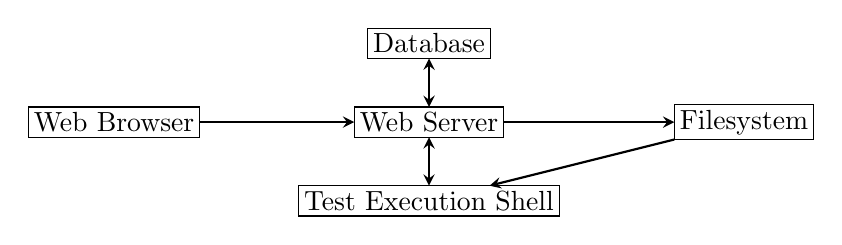
\begin{tikzpicture}
\tikzstyle{arrow} = [thick,->,>=stealth]
\tikzstyle{darrow} = [thick,<->,>=stealth]
\tikzstyle{actor} = [draw,outer sep=0,inner sep=2, minimum size=10]

\node(browser)[actor]{Web Browser};
\node(server)[actor, right of=browser, node distance=4cm]{Web Server};
\node(filesystem)[actor, right of=server, node distance=4cm]{Filesystem};
\node(db)[actor, above of=server, node distance=1cm]{Database};
\node(shell)[actor, below of=server, node distance=1cm]{Test Execution Shell};
 
\draw [arrow] (browser) -- node[midway, auto] {} (server);
\draw [arrow] (server) -- node[midway, auto] {} (filesystem);
\draw [arrow] (filesystem) -- node[midway, auto] {} (shell);
\draw [darrow] (server) -- node[midway, auto] {} (db);
\draw [darrow] (server) -- node[midway, auto] {} (shell);
\end{tikzpicture}
\end{figure}
The basic system architecture that will be used is as follows: The website will use a client-server model, with the student/teacher's web browser acting as the client. The web server will store any submissions on the filesystem, as well as test results. The server will also contact a shell to run the submitted tests on solutions. In addition to this, a database may be required to assist in tracking which submissions are uploaded, where they are stored, etc.

\section{Sequence of Operations}
This diagram provides an overview for how a student might interact with with the final, implemented, system. It describes the sequence of operations and messages between actors inside the system, in various situations. This diagram is an early overview of a possible implementation, and will likely be different to the final implementation. This diagram also omits the database and focuses more on interactions related to the functionality users will see.\\
\begin{sequencediagram}
\newthread{u}{User}
\newinst[2]{i}{Interface}
\newinst[2]{f}{Files}
\newinst[2]{s}{Shell}

\begin{sdblock}{Submission}{}
    \begin{call}{u}{Submit solution}{i}{ready}
        \begin{call}{i}{Store solution}{f}{errors?}
        \end{call}
    \end{call}
\end{sdblock}

\begin{sdblock}{Test Submit}{}
\begin{messcall}{u}{Submit test}{i}{ready}
    \begin{call}{i}{Store test}{f}{errors?}
    \end{call}
\mess[1]{i}{ready}{u}
\begin{call}{i}{Execute test}{s}{result}
    \begin{call}{s}{Get solution and test}{f}{files}
    \end{call}
\end{call}
\begin{call}{i}{Store result}{f}{errors?}
\end{call}
\end{messcall}

\end{sdblock}
\end{sequencediagram}

%   _____  _____   ____       _            __  __          _   _ 
%  |  __ \|  __ \ / __ \     | |          |  \/  |   /\   | \ | |
%  | |__) | |__) | |  | |    | |  ______  | \  / |  /  \  |  \| |
%  |  ___/|  _  /| |  | |_   | | |______| | |\/| | / /\ \ | . ` |
%  | |    | | \ \| |__| | |__| |          | |  | |/ ____ \| |\  |
%  |_|    |_|  \_\\____/ \____/           |_|  |_/_/    \_\_| \_|

\chapter{Project Management}
\section{Timetable}
The following hard deadlines exist for the project:\\
\begin{tabularx}{\textwidth}{lX}
\textbf{Date} & \textbf{Task}\\
24 Nov 2016 & First Deliverable submitted as a PDF through Vision\\
25 Nov 2016 & Ethics approval submission made through project system\\
16 Dec 2016 & Interview with supervisor and second reader completed\\
17 Mar 2017 & Draft dissertation to supervisor for written feedback\\
24 Apr 2017 & Dissertation submitted\\
. & Dissertation submitted as a PDF through Vision\\
. & Dissertation and ZIP file of all files submitted through Project System\\
 5 May 2017 & Poster uploaded through Vision\\
. & Edinburgh Poster Session
\end{tabularx}
\subsection*{Implementation Targets}
In addition to the above imposed timetable limits, I have arranged some self-imposed targets. These are included in the Gantt chart located in the appendices, and relate to targets of which requirements need to implemented and when. As I am just one developer, most of the functionality will be implemented in series rather than parallel, but some points (such as uploading files) can be developed together. The first item developed will be a basic website with interfaces available to plug in the various other features, as they are implemented.

\section{Risk management}
This section details some of the risks involved during the project, their likelihood, and a description of possible mitigation and recovery strategies.\\
The following scales are used when measuring likelihood:\par
{\centering
\begin{tabular}{c|c|c|c|c}
Very Unlikely & Unlikely & Possible & Likely & Very Likely
\end{tabular}\par\noindent}
And also the impact such a risk occurring would have on the project:\par
{\centering
\begin{tabular}{c|c|c|c|c}
 No Impact & Small Impact & Some Impact & Big Impact & Large Impact\\
 Negligible & ... & ... & ... & Project may fail
\end{tabular}\par\noindent}
\riskitem{Eval}{Not enough users for evaluation}{Likely, Big Impact}{It may be the case that I am not able to get a substantial number of participants during the evaluation. In this event, I may offer more incentives to get participants and request more detailed information from them when discussing the evaluation.}
\riskitem{No-Impl}{No usable implementation for evaluation}{Unlikely, Big Impact}{I may be unable to complete a usable implementation in time for the evaluation. If I suspect this is the case beforehand, I will scale back the scope and focus on implementing core functionality. In the worst case, a wizard-of-oz style system could be set up at the last minute.}
\riskitem{Loss}{Work (Code or otherwise) is lost}{Possible, Big Impact}{During development of the application, or write-up of a report, work done might become lost, corrupted or overwritten. To prevent this version control is used, and work is also backed up across a development machine (personal), deployment machine (University server) and cloud storage (GitHub.com). Should one of the sources be lost, the others should still be usable.}
\riskitem{Wares}{Software that is needed does not work}{Possible, Large Impact}{A software package that the implementation relies upon is unable to meet the requirements, or has bugs, or simply does not work. To prevent this, possible packages should be thoroughly researched before choosing. If the problems are discovered later, an alternate package could be chosen, or the functionality offered by this could be scaled back or removed.}
\riskitem{Meet}{Cannot meet with supervisor}{Likely, Small Impact}{There may come a time when I, or the project supervisor are unable to meet and discuss recent developments or issues that have arisen. This may be due to travel, weather etc. In such an event, communication could be done via. email. Given that there is a timetable and plan for this project, I would continue to follow this until such a time as a full meeting could be arranged.}
\section{Issues}
To my knowledge, there are no legal issues that might arise from the implementation of this project. However, the data collected during the evaluation will need to be kept anonymous. I will make every effort to keep this information secure once it is collected, and include a method such that I, and only I, may identify and remove participants results if they wish this to happen at a later date.\par
In terms of social and ethical issues, students may be affected. During the evaluation, as the test subjects are students, they will be taking part in the evaluation mid-semester. It is important that the impact of having taken part in the evaluation not have an adverse effect on their performance in classes or other coursework. To support this, it will be made clear to participants that their grades will not be affected by taking part, and make it clear that students can withdraw at their own wish.\par
During both the evaluation and implementation, I will act in a professional manner that is consistent with what is expected by the university: Giving credit for help where it is due, treating people with respect, and being truthful in what I report.

\singlespacing
\printbibliography

\addcontentsline{toc}{chapter}{Appendices}
\addcontentsline{toc}{section}{Gantt Chart}
\begin{landscape}
\includepdf[pages={2,3},angle=90]{../Gantt.pdf}
\end{landscape}

\addcontentsline{toc}{section}{Ethical Analysis}
\section*{Ethical Analysis}
\textbf{Student}: L\'eon McGregor\\
\textbf{Title}: Web platform for code peer-testing\\
\textbf{Supervisor}: Manuel Maarek\\
\textbf{Abstract}: Develop a web platform for managing peer-testing and peer-feedback of programming code. The project aims at providing a user-friendly solution for giving and receiving feedback on programming artifacts.\\
\textbf{Purpose of Study}: The purpose of this study is to investigate the effectiveness of a prototype web platform for peer assessment of programming code. The test subjects will be asked to perform small programming exercises, and peer assess each others work. The test subjects will attempt this without and then with the prototype website, in order to see if the website is effective. Test subjects will also be given some questionnaires to fill out, and may participate in an extended discussion session if they choose.

\subsection*{Screening}
\textbf{Does the research involve any of the following?}: Human Subjects\\
\textbf{Interface Only Screening?}: No\\
\textbf{Full Ethical Screening?}: Other body not required

\subsection*{Use of Human Subjects}
\textbf{How will participants be recruited?}: Participants will ideally be students of computer science at Heriot-Watt. A general request for participants to join in will be sent out, perhaps through a university emailing list, or by posting flyers. This will be done up to a week before the study is conducted.\\
\textbf{All participants to be recruited are over 16, able to give informed consent, and have no known impediment that might affect their ability to participate in the study?}: Yes\\
\textbf{How long will participants have to decide whether to take part in the study?}: 7 Days\\
\textbf{Does the study involve actively deceiving participants?}: No\\
\textbf{Will participants be using non-standard hardware?}: No

\subsection*{Data Protection Compliance}
I confirm that, in accordance with Data Protection legislation:
\begin{itemize}
\item Indentifiable data will be stored on a secure machine with restricted access
\item Data will be anonymised before publication unless consent has been given
\item Identifiable data will only be retained for the duration of the consent granted by the participant
\item External data and systems will be used within the licence terms specified
\end{itemize}

\subsection*{Health and Safety}
I confirm that the project involves only standard IT equipment and exposes participants to no more hazards than a conventional office environment.

\end{document}
